% !TEX root = report.tex
%============================================================================================
\newpage
\section{Robust PCA with known rank: a block coordinate descent approach}

%-----------------------------------------------------------------------------------------------------------------------------------------------------------------
\subsection{Motivation}
In some applications we may have some prior information about the low rank component of an observed matrix. For example, in computer vision, if we were to extract the background from different frames of a video, then it is natural to consider each video frame as a long vector (by stacking its columns). The background that we are recovering is then a single vector, which means that the associated component in the matrix collecting the frames is of rank 1. Therefore, it is a very natural question to ask whether we can utilize this additional rank information to derive faster or more scalable algorithms while retaining the performance guarantees of Robust PCA.



%-----------------------------------------------------------------------------------------------------------------------------------------------------------------
\subsection{Equivalent formulation of Robust PCA with rank information}

We first show the intuitive fact that within the robust PCA framework, the same probability guarantee will still hold when additional information on the problem is incorporated as constraints to the optimization problem. Then we derive a block-coordinate descent algorithm for the case when rank information is known.
\begin{prop}
\label{prop:restriction prob}Let $M=L_{0}+S_{0}$ , $rank(L_{0})\le r$ and $(L_0,S_0)$
satisfy the Robust PCA assumptions. Then with high probability, the
following problems are equivalent:
%
\begin{eqnarray}
J_{1} & =\min_{L,S} & \|L\|_{*}+\lambda\|S\|_{1}\label{eq:general}\\
 & s.t. & M=L+S\nonumber
\end{eqnarray}
%
\begin{eqnarray}
J_{2} & =\min_{L,S} & \|L\|_{*}+\lambda\|S\|_{1}\label{eq:restricted}\\
 & s.t. & M=L+S\nonumber \\
 &  & \text{and }\;T(L,S)\text{ holds}\nonumber
\end{eqnarray}
%
where $T(L,S)$ are conditions on $(L,S)$ that $(L_{0},S_{0})$ also
satisfies.
\end{prop}

\begin{proof}
We use subscript to denote the optimizer for $J_{1}$ and $J_{2}$ respectively.
With high probability, $(L_{1},S_{1})=(L_{0},S_{0})$. Now, over the event of $(L_{1},S_{1})=(L_{0},S_{0})$, $(L_{1},S_{1})$ is also a feasible solution for (\ref{eq:restricted}). Since $J_{1}\le J_{2}$ always, now $(L_{1},S_{1})$ achieve the bound for (\ref{eq:restricted}).
Note that it should also be unique because otherwise it would contradict with the recovery of (\ref{eq:general}).
\end{proof}

Now we apply Proposition (\ref{prop:restriction prob}) to the case when the rank information is known and derive a block coordinate descent algorithm.

Consider the problem
\begin{alignat}{3}
J_{3}
&= &&\min_{L, S}  && \|L\|_{*} + \lambda \|S\|_{1} \notag \\
&&&\text{s.t.} && M=L+S, \ \text{rank}(L)\le r \notag \\
&= &&\min_{L, S, p_i, q_i, \mu_i} && \|L\|_{*} + \lambda\| M - L \|_{1} \notag \\
&&& \text{s.t.} && L = \sum_{i=1}^{r} \mu_{i}p_{i}q_{i}^{T}, \  p_i^Tp_j = \delta_i^j, \ q_{i}^Tq_j = \delta_i^j, \ \mu_{i}\ge0 \notag \\
&= && \min_{\mu_{i}, p_{i}, q_{i}} && \sum_{i=1}^{r} \mu_{i} + \lambda \|M - \sum_{i=1}^{r} \mu_{i}p_{i}q_{i}^{T}\|_{1} \notag \\
&&& \text{s.t.} && p_i^Tp_j = \delta_i^j, \ q_{i}^Tq_j = \delta_i^j, \mu_{i} \ge 0 \notag \\
& = && \min_{\mu_{i}, p_{i}, q_{i}} && \sum_{i=1}^{r} |\mu_{i}| + \lambda \|M - \sum_{i=1}^{r} \mu_{i} p_{i} q_{i}^{T}\|_{1} \label{eq:rank form} \\
&&& \text{s.t.} && p_i^Tp_j = \delta_i^j, \ q_{i}^Tq_j = \delta_i^j, \ \mu_{i} \ge 0 \notag
\end{alignat}

Here $L = \sum_{i=1}^{r} \mu_{i}p_{i}q_{i}^{T}$ is the SVD of $L$, hence the condition of orthonormality $p_i^Tp_j = \delta_i^j, \ q_{i}^Tq_j = \delta_i^j$. Note that this formulation allows us to optimize over $\mu_{i}$, $p_{i}$ and $q_{i}$ sequentially. By Proposition~\ref{prop:restriction prob}, we know that the formulation of~\eqref{eq:rank form} can recover the original pair $(L_{0},S_{0})$ with high probability.


%-----------------------------------------------------------------------------------------------------------------------------------------------------------------
\subsection{Simplification using $\ell_{1}$ heuristic}


%------------------------------------------------------------------------------
\subsubsection{Introduction}

Recall that the nuclear norm is used in the PCP scheme as a heuristic to recover a low rank component corrupted by gross random noise. The nuclear norm is used because it penalizes high rank matrices and encourages sparsity of the vector of singular values. Now, we consider the case when we have additional information about the rank of the low-rank matrix~$L$. Assume the rank of the matrix is known. Since information about the rank of the matrix is available, one can replace the nuclear norm heuristic by writing $L$ in the form $L = \sum_{j = 1}^r p_j q_j^T$. This guarantees $\mathbf{rank}(L) \leq r$. Note that $p_j$'s and $q_j$'s do not necessarily give the directions of the singular vectors of $L$, since they are not assumed to be orthogonal. This results in the following heuristic

\begin{eqnarray}
E^{*} & = & \min_{\{p_{j}\}\{q_{j}\},1\le j\le r}\|M-\sum_{j=1}^{r}p_{j}q_{j}^{T}\|_{1}\label{heu}
\end{eqnarray}



%------------------------------------------------------------------------------
\subsubsection{Performance guarantee for the $\ell_1$ heuristic}

For this new heuristic, we provide some performance guarantee for the case when the noise is bounded. One is a result for deterministic case
and the other is for the random case. They are as follows.

\begin{prop}
Let $M=S+\sum_{i=1}^{r}p_{i}q_{i}^{T}$ and $\frac{2}{\epsilon}\|S\|_{1}\le\|\sum_{i=1}^{r}p_{i}q_{i}^{T}\|_{1}$. Then, the estimate $\hat{L}$ recovered from~\eqref{heu} satisfies
\begin{eqnarray*}
\frac{\|\sum_{i=1}^{r}p_{i}q_{i}^{T}-\hat{L}\|_{1}}{\|\sum_{i=1}^{r}p_{i}q_{i}^{T}\|_{1}} & \le & \epsilon
\end{eqnarray*}
\end{prop}
\begin{proof}
Suppose not, then
\begin{eqnarray*}
\|S\|_{1} & \ge & \|\sum_{i=1}^{r}p_{i}q_{i}^{T}+S-\hat{L}\|_{1}\\
 & \ge & \|\sum_{i=1}^{r}p_{i}q_{i}^{T}-\hat{L}\|_{1}-\|S\|_{1}\\
 & > & \epsilon\|\sum_{i=1}^{r}p_{i}q_{i}^{T}\|_{1}-\|S\|_{1}
\end{eqnarray*}
which contradicts the assumption that
\begin{eqnarray*}
\frac{2}{\epsilon}\|S\|_{1} & > & \|\sum_{i=1}^{r}p_{i}q_{i}^{T}\|
\end{eqnarray*}
\end{proof}
%This gives a contraditcion, which is,
%\begin{eqnarray*}
%\frac{2}{\epsilon}\|S\|_{1} & > & \|\sum_{i=1}^{r}p_{i}q_{i}^{T}\|
%\end{eqnarray*}

\begin{prop}
Let $M=\sum_{i=1}^{r}p_{i}q_{i}^{T}+S$, where $S_{i,j}\sim Uniform(-x_{s},x_{s})$,
$(p_{i})_{j}\sim Uniform(-x_{p},x_{p})$, $(q_{i})_{j}\sim Uniform(-x_{q},x_{q})$, where all random variables are independent. With $|S|=k$ such that
$\lim_{n\to\infty}\frac{k^{2}}{n}$, then we have,
\[
\lim_{n \to \infty} P \left( \frac{ \|\sum_{i=1}^{r} p_{i} q_{i}^{T} - \hat{L} \|_{1} }{ \| \sum_{i=1}^{r} p_{i} q_{i}^{T} \|_{1} } > \epsilon \right) = 0
\]
\end{prop}

\begin{proof}
Let $E$ be the error event that $\frac{\|\sum_{i=1}^{r}p_{i}q_{i}^{T}-\hat{L}\|_{1}}{\|\sum_{i=1}^{r}p_{i}q_{i}^{T}\|_{1}}>\epsilon$.
If error occurs,
\begin{eqnarray*}
kx_{s} & \ge & \|\sum_{i=1}^{r}p_{i}q_{i}^{T}+S-\hat{L}\|_{1}\\
 & \ge & \|\sum_{i=1}^{r}p_{i}q_{i}^{T}-\hat{L}\|_{1}-\|S\|_{1}\\
 & \ge & \epsilon\|\sum_{i=1}^{r}p_{i}q_{i}^{T}\|_{1}-kx_{s}\\
 & \ge & \epsilon\sqrt{\sum_{l_{1}l_{2}}(\sum_{i=1}^{r}(p_{i})_{l_{1}}(q_{i})_{l_{2}})^{2}}-k_{s}
\end{eqnarray*}


Thus,
\begin{eqnarray*}
Pr(E)
&\le & Pr \left( \left( \frac{2kx_{s}}{\epsilon} \right)^{2} \ge \sum_{l_{1}l_{2}} \left( \sum_{i=1}^{r}(p_{i})_{l_{1}}(q_{i})_{l_{2}} \right)^{2} \right)\\
&\le & Pr \left( \left( \frac{2kx_{s}}{\epsilon} \right)^{2} \ge \sum_{l_{1}=1}^{n} \left( \sum_{i=1}^{r}(p_{i})_{l_{1}}(q_{i})_{l_{1}} \right)^{2} \right)\\
&= & Pr \left( \frac{1}{n} \left( \frac{2kx_{s}}{\epsilon} \right)^{2} \ge \frac{1}{n} \sum_{l_{1}=1}^{n} \left( \sum_{i=1}^{r}(p_{i})_{l_{1}}(q_{i})_{l_{1}} \right)^{2} \right)
\end{eqnarray*}


Moreover, as $E(\sum_{i=1}^{r}(p_{i})_{l_{1}}(q_{i})_{l_{1}})^{2})=\frac{r}{3}x_{p}^{2}x_{q}^{2}$,
by the law of large numbers, $\frac{1}{n}\sum_{l_{1}=1}^{n}(\sum_{i=1}^{r}(p_{i})_{l_{1}}(q_{i})_{l_{1}})^{2})\to\frac{r}{3}x_{p}^{2}x_{q}^{2}$.
Thus, since $\frac{1}{n}(\frac{2kx_{s}}{\epsilon})^{2}\to0$. This
gives $Pr(E)\to0$ as $n\to\infty$.
\end{proof}

However, we know that the $\ell_1$ heuristic cannot work well in the case of unbounded noise. This can be seen from the following example. Say, for $n=100$, 
\begin{alignat*}{2}
L_{0}&=\begin{bmatrix} 1\\ 1\\ \vdots \\ 1\end{bmatrix} \begin{bmatrix} 1 & 1 & \dots & 1 \end{bmatrix}, &\qquad \qquad
S_{0} &= \begin{bmatrix} 10^{9} & 0 & \dots & 0\\  0 & 0 & \dots & 0\\ \vdots & \vdots &  & \vdots\\ 0 & 0 & \dots & 0
\end{bmatrix}
\end{alignat*}
%
then by the $\ell_{1}$ heuristic, we would get 
\begin{alignat*}{2}
\hat{L}_{0}&=\begin{bmatrix} 10^9\\ 1\\ \vdots \\ 1\end{bmatrix} \begin{bmatrix} 1 & 10^{-9} & \dots & 10^{-9} \end{bmatrix}, &\qquad \qquad
\hat{S}_{0} &= \begin{bmatrix} 1 & 0 & \dots & 0\\  0 & 1 & \dots & 1\\ \vdots & \vdots &  & \vdots\\ 0 & 1 & \dots & 1
\end{bmatrix}
\end{alignat*}
%
which deviates grossly from the original pair. However, Robust PCA can achieve exact recovery even in this case because it penalize the nuclear norm of~$L$.



%-----------------------------------------------------------------------------------------------------------------------------------------------------------------
\subsection{A block coordinate descent algorithm}

For simplicity we restrict our discussion to $r=1$ in~\eqref{heu}. Let $M=(M_{i,j})\in R^{n \times m}$. The problem is then
%
\[
\begin{aligned}
\min_{p \in \Rbb^n, q \in \Rbb^m} \|M - pq^T\|_1 &&\text{subject to } \|p\|_\infty = 1
\end{aligned}
\]
One can use a block coordinate descent algorithm, similar to power iteration, by iteratively fixing one vector and optimizing on the other. 

%------------------------------------------------------------------------------
\subsubsection{$q$-step} For a fixed $p \in \Rbb^n$, the problem is
\[
\min_{q \in \Rbb^m} \sum_{j = 1}^m \|M_j - q_jp\|_1 = \sum_{j = 1}^m \min_{q_j} \|M_j - q_jp\|_1
\]
where $M_j \in \Rbb^n$ is the $j$-th column of $M$. Each subproblem is an $\ell_1$-norm projection (projection of $M_j$ onto $\text{span}(p)$)
\[
\min_t \|z - tp\|_1
\]

This is a weighted median problem $\min_t \|z - tp\|_1 \Leftrightarrow \min_t \sum_{i \in \text{supp(p)}} |p_i| \left| \frac{z_i}{p_i} - t \right| $.

%------------------------------------------------------------------------------
\subsubsection{Median problem}
The median problem is
\[
\min_t \sum_{i = 1}^n |z_i - t|
\]
and an optimizer is $t = z_{[k]}$ where $z_{[i]}$ is the $i$-th element in the ordered sequence, $k$ is the maximum index such that $k \leq n-k$ i.e. $\lfloor \frac{n}{2} \rfloor \leq k \leq \lceil \frac{n}{2} \rceil$. This can be solved by simply sorting the elements of $z$, which can be done in $O(n \log n)$.

Note that computing the median can be done in $O(n)$ if the elements are not sorted entirely: using the quick-select algorithm, a modified version of the quicksort algorithm. At each step, assume we have a list of $k$ elements. We choose a random pivot, and in one pass compute the elements that are less than, respectively greater than, the pivot. From the length of each list, we know where to look for the median next. If the sizes of the sublists are sufficiently balanced, this will result in $O(n)$ algorithm. In the exactly balanced case, the complexity is proportional to $n + \frac{n}{2} + \frac{n}{4} + \dots + \frac{n}{\log_2 n} = n\frac{1-(1/2)^{1 + \log_2 n}}{1 - 1/2} \leq 2n$. In the case the size of each sublist is no less than $\alpha$ times the size of the parent list, the complexity is also linear, since it is proportional to $n + \alpha n + \alpha^2 n + \dots + \alpha^{\log_{1/\alpha} n} n \leq \frac{1}{1 - \alpha}n$. 
Although the worst-case complexity is $O(n^2)$, the algorithm is linear in practice. Assuming a uniform distribution of the permutation that will result in the sorted list, the expected complexity is $O(n)$.


%------------------------------------------------------------------------------
\subsubsection{Weighted median problem}
The solution to the weighted median problem is slightly different
\[
\min_t \sum_{i = 1}^n \alpha_j |z_i - t|
\]
where $\alpha_i > 0$. An optimizer is $t = z_{[k]}$ where $k$ is the maximum index such that $\sum_{i = 1}^k \alpha_i \leq \sum_{i = k+1}^n \alpha_i$.  This is shown by using the property of sub-differential of $\|.\|_{1}$ and by noting that $0 \in \partial (\sum_{i = 1}^n \alpha_j |z_i - t|)$ for $t = z_{[k]}$. Finding this optimal $t$ can also be achieved by sorting.

If we denote this subproblem by
\begin{align*}
\mathbf{wmed}(M, p) 
&= \arg \min_t \|M - pt^T\|_1 \\
&= \arg \min_t \sum_{j} \|M_j - t_jp\|_1 \\
&= \arg \min_t \sum_{j} \sum_{i \in \mathbf{supp}(p)} |p_i| \left| \frac{M_{ij}}{p_i} - t_j \right|
\end{align*}
where $M_j$ is the $j$-th column of $M$, then the $q$-step is simply given by
\[
q \leftarrow \mathbf{wmed}(M, p) 
\]
and the complexity of the $q$-step is $O(mn\log n)$. The $\mathbf{wmed}$ algorithm is summarized in Algorithm~\cite{wmhalgo}.
%
\begin{algorithm}[h]
\KwIn{Data matrix~$M$, vector~$p$}
\For{$j \in \{1, \dots, m\}$}{
\begin{enumerate}
\item Define vectors $z$ and $\alpha$: $\forall i \in \mathbf{supp}(p)$, $\alpha_i = |p_i|$ and $z_i = \frac{M_{ij}}{p_j}$.
\item Sort $z$ s.t. $z_{i_{1}} \le z_{i_{2}} \le \dots \le z_{i_n}$
\item Find the maximum $k$ s.t. $\sum_{l = 1}^k \alpha_{i_l} \leq \sum_{l = k+1}^n \alpha_{i_l} $
\item Set $q_j = z_{i_k}$
\end{enumerate}
}
\KwOut{vector~$q$}
\caption{q = $\mathbf{wmed}(M,p)$}
\label{wmhalgo}
\end{algorithm}

%------------------------------------------------------------------------------
\subsubsection{$p$-step} 
For a fixed $q \in \Rbb^m$, the problem is given by
\[
\min_{\|p\|_\infty = 1} \sum_{i = 1}^n \|M_i - p_i q\|_1
\]
where $M_i$ is the $i$-th row of $M$. We can denote this problem by
\[
p \leftarrow \mathbf{cwmed}(M^T, q)
\]

where $\mathbf{cwmed}(M^T, q)$ is the solution of the constrained weighted median problem
\[
\min_{\|p\|_\infty = 1} \sum_{i} \|M_i - p_i q\|_1 = \sum_{i = 1}^n \min_{|p_i| \leq 1} \|M_i - p_i q\|_1 \text{ subject to } \max_i |p_i| = 1
\]

  

We can start by solving $n$ constrained weighted median problems $\min_{|p_i| \leq 1} \|M_i - p_i q\|_1$. This is solved by computing the solution to the unconstrained weighted median 
\[
p_i = \arg \min_{t_i} \sum_{j \in \text{supp}(q)} |q_j| \left| \frac{M_{ij}}{q_j} - t_i \right|
\]
then projecting $p_i$ on $[-1, 1]$.

After solving the $n$ subproblems, there are 2 cases. Either one of the $p_i$'s satisfies $|p_i| = 1$, in which case the $\|p\|_\infty = 1$ constraint is satisfied and the problem is solved, or all the $p_i$'s are such that $|p_i| < 1$. In this case, we choose which $p_i$ to project on $[-1, 1]$ by solving the problem
\begin{equation}
\label{p_step_projection}
\begin{aligned}
&\text{minimize}_{i,\epsilon} && -\|M_i - p_i q\|_1 + \|M_i - \epsilon q\|_1 \\
& \text{subject to} 
&& i \in \{1, \dots, n\} \\
&&& \epsilon \in \{-1, 1\}
\end{aligned}
\end{equation}
this problem finds $(i, \epsilon)$ that minimize the increase of the objective value that is due to setting $p_i = \epsilon$. Then if $(i_0, \epsilon_0)$ is a minimizer, we set $p_{i_0} = \epsilon_0$. This additional projection step is $O(nm)$ since there are $2n$ feasible points to evaluate in problem~(\ref{p_step_projection}). The $\mathbf{cwmed}$ algorithm can be summarized by Algorithm~\ref{alg:cwmed}

\begin{algorithm}[h]
\KwIn{Data matrix~$M$, vector~$q$}
\For{$i \in \{1, \dots, n\}$}{
\begin{enumerate}
\item Define vectors $z$ and $\alpha$: $\forall j \in \mathbf{supp}(q)$, $\alpha_j = |q_j|$ and $z_j = \frac{M_{ij}}{p_i}$.
\item Sort $z$ s.t. $z_{j_{1}} \le z_{j_{2}} \le \dots \le z_{j_n}$
\item Find the maximum $k$ s.t. $\sum_{l = 1}^k \alpha_{j_l} \leq \sum_{l = k+1}^n \alpha_{j_l} $
\item Set $p_i = z_{j_k}$
\item Project $p_i$ on $[-1, 1]$
\end{enumerate}
}
\If{$\|p\|_\infty < 1$}{
\begin{enumerate}
\item Let $(i_0, \epsilon_0) = \arg \min_{i,\epsilon} -\|M_i - p_i q\|_1 + \|M_i - \epsilon q\|_1$
\item Set $p_{i_0} = \epsilon_0$
\end{enumerate}
}
\KwOut{vector~$p$}
\caption{$\mathbf{p = cwmed}(M^T,q)$}
\label{alg:cwmed}
\end{algorithm}


%------------------------------------------------------------------------------
\subsubsection{Algorithm for the constrained problem} 
The Constrained rank one $\ell_1$ heuristic is given in Algorithm~\ref{alg:l1_heur_const}
\begin{algorithm}[h]
\While{not converged}{
\[
\begin{aligned}
&q \leftarrow \mathbf{wmed}(M, p) \\
&p \leftarrow \mathbf{cwmed}(M^T, q)
\end{aligned}
\]
}
\caption{Constrained rank one $\ell_1$ heuristic}
\label{alg:l1_heur_const}
\end{algorithm}

The complexity of each iteration is $O(nm\log (nm))$ if the weighted median is computed by sorting the vectors, or $O(nm)$ if the quick select algorithm is used instead. 
It is important to point out that while the~$\ell_1$ heuristic enjoys recovery guarantees, we have no guarantee that this iterative algorithm will converge to an optimizer of the problem. However, we observe that this heuristic performs well in practice when the low rank component $L$ is rank one. We also observe that solving an unconstrained version of the problem, where vectors $p$ and $q$ are normalized at each iteration, works better in practice. An example simulation is shown in Figure~\ref{fig:l1pca_const_vs_proj}, where a simulation was run using randomly generated rank-one $10 \times 10$ matrices, corrupted with random noise matrices with increasing support. For each support size, $20$ simulations are run. The plots show the average results.

\begin{figure}[h!]
\centering
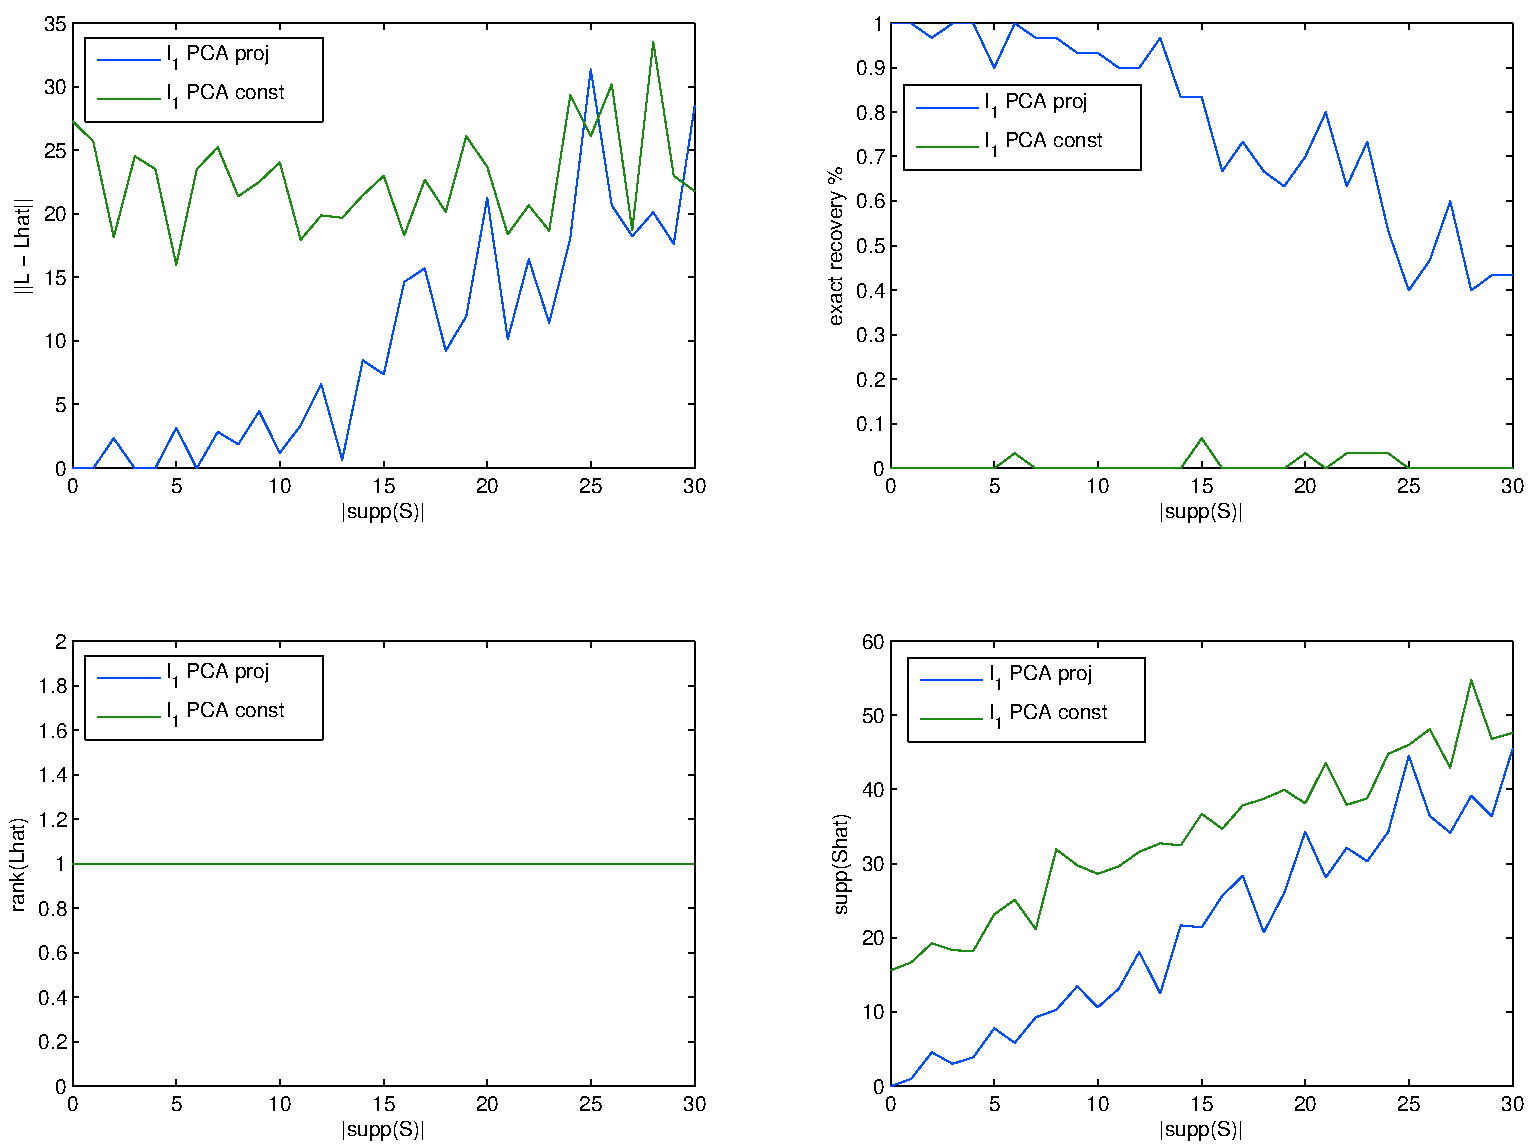
\includegraphics[width=\textwidth]{../figures/l1pca_proj_vs_const.pdf}
\label{fig:l1pca_const_vs_proj}
\caption{Performance of the constrained $\ell_1$ PCA heuristic (green) Vs. the projected $\ell_1$ PCA heuristic (blue), for increasing size of the support of the corruption matrix $S$. The projected method performs considerably better (higher exact recovery rate, lower average $\ell_1$ error, support size of the recovered $\hat{S}$ closer to the original support).}
\end{figure}

\newpage
The unconstrained version is detailed next.

\subsubsection{Algorithm for the unconstrained projected problem} 
Another approach is to apply block coordinate decent to the unconstrained problem
\[
\begin{aligned}
\min_{p \in \Rbb^n, q \in \Rbb^m} \|M - pq^T\|_1
\end{aligned}
\]
but project the vectors at each iteration. This results in Algorithm~\ref{alg:l1_heur_proj}

\begin{algorithm}[h]
\While{not converged}{
\[
\begin{aligned}
&q \leftarrow \mathbf{wmed}(M, p) \\
&q \leftarrow q / \|q\|_\infty \\
&p \leftarrow \mathbf{wmed}(M^T, q)\\
&q \leftarrow p / \|p\|_\infty
\end{aligned}
\]
}
\caption{Projected rank one $\ell_1$ heuristic}
\label{alg:l1_heur_proj}
\end{algorithm}

The complexity of each iteration is $O(nm\log (nm))$ if the weighted median is computed by sorting the vectors, or $O(nm)$ if the quick select algorithm is used instead.


%------------------------------------------------------------------------------
\subsubsection{convergence in the rank one case}
Note on convergence when there is no noise. Assume $A$ is rank one (no observation noise), and let $A = \sigma uv^T$ where $\sigma > 0$, $u$ and $v$ are unit vectors.

Then the $p$-step is given by
\begin{align*}
p_i 
&= \arg \min_{p_i} \|\sigma u_i v - p_iq\|_1 \\
&= \arg \min_{p_i} \sum_{j = 1}^n |\sigma u_i v_j - p_iq_j| \\
&= \arg \min_{p_i} \sum_{j = 1}^n |q_j| \left| \frac{\sigma u_i v_j}{q_j} - p_i \right| \\
&= \sigma u_i \tilde{v}_{[k]}
\end{align*}

where $\tilde{v}_i = \frac{v_i}{q_i}$, $\tilde{v}_{[k]}$ is the $k$-th element in the ordered sequence of $\tilde{v}$. Note that the sign of $u_i$ does not affect the solution, even though it may seem to affect the order of the sequence: if $u_i < 0$, simply write the optimization problem as $\min_{p_i} \|\sigma u_i v - p_iq\|_1 = \min_{p_i} \|\sigma (-u_i) v - (-p_i)q\|_1$ where now $-u_i > 0$ and the variable is $-p_i$. The solution in the positive case yields  $-p_i = \sigma (-u_i) \tilde{v}_{[k]}$, which is the same as $ p_i = \sigma u_i \tilde{v}_{[k]}$.

Therefore we have that after the first iteration, 
\[
p = \tilde{v}_{[k]} u
\]
since $\tilde{v}_{[k]}$ does not depend on $i$ (the order of the sequence only depends on $q$), thus we immediately recover the direction of the left singular vector $u$. Similarly, $q$ recovers the direction of the right singular vector $v$, and the algorithm converges after one iteration. This is observed in practice (however since the stopping needs to detect that the vectors are not changing, this requires two iterations in practice).



%-----------------------------------------------------------------------------------------------------------------------------------------------------------------
\subsection{Sensitivity of the Robust PCA solution to $\lambda$}

Note that in the Robust PCA framework, the parameter $\lambda$ is specifically chosen to be $\lambda = \frac{1}{\sqrt{n}}$, and when $\lambda$ is too large or too small, it would significantly affect the recovery. However, in the case where rank information is given, the effect of $\lambda$ may be different. One may ask whether recovery can be be guaranteed with very small values of $\lambda$. In particular, we specialize to the rank 1 case, and it turns out that it cannot be done, as demonstrated in the following.

Recall that if we directly apply Robust PCA we will get

\begin{align*}
 \min_{M=L+S,rank(L)\le1}\|L\|_{*}+\lambda\|S\|_{1}
 & = \min_{S=M-pq^{T},L=pq^{T}}\|L\|_{*}+\lambda\|S\|_{1} \\
 & = \min_{S=M-pq^{T},L=pq^{T}}\|pq^{T}\|_{*}+\lambda\|M-pq^{T}\|_{1} \\
 & = \min_{p,q:\|p\|_{2}=1}\|pq^{T}\|_{*}+\lambda\|M-pq^{T}\|_{1} \\
 & = \min_{p,q:\|p\|_{2}=1}\|q\|_{2}+\lambda\|M-pq^{T}\|_{1} \\
 & = \min_{p:\|p\|_{2}=1}\min_{q}\|q\|_{2}+\lambda\|M-pq^{T}\|_{1}
\end{align*}


Now, for every fixed $p$, consider the subproblem of directly
applying Robust PCA with $\lambda\le\frac{1}{n}$,

\begin{align*}
\min_{q}\|q\|_{2}+\lambda\|M-pq^{T}\|_{1}
& = \min_{q}\max_{\|u\|_{2}\le1,\|V\|_{\infty\le1}}u^{T}q+\lambda Tr(V^{T}(M-pq^{T})) \\
& = \max_{\|u\|_{2}\le1,\|V\|_{\infty\le1}}\min_{q}u^{T}q+\lambda Tr(V^{T}(M-pq^{T})) \\
& = \max_{\|u\|_{2}\le1,\|V\|_{\infty\le1},u=\lambda V^{T}p} \lambda Tr(V^{T}M) \\
& = \max_{\|\lambda V^{T}p\|_{2}\le1,\|V\|_{\infty\le1}} \lambda Tr(V^{T}M) \\
& = \max_{\|V^{T}p\|_{2}\le n,\|V\|_{\infty\le1}} \lambda Tr(V^{T}M)
\end{align*}


Now note that, since $\|p\|_{2}\le1$, we have $\|V^{T}p\|_{2}\le\sqrt{\sum_{i=1}^{n}\sigma_{i}(V^{T}V)}=\sqrt{Tr(V^{T}V)}\le\sqrt{n^{2}\|V\|_{\infty}}$.
Thus, the optimal value is
\begin{align*}
\min_{p,q:\|p\|_{2}=1}\|pq^{T}\|_{*}+\lambda\|M-pq^{T}\|_{1}
& = \min_{p:\|p\|_{2}=1}\max_{\|V\|_{\infty\le1}}\lambda Tr(V^{T}M)\\
& = \lambda \min_{p:\|p\|_{2}=1}\|M\|_{1}\\
& = \lambda \|M\|_{1}
\end{align*}


And it is achieved by $pq^{T}=0$ matrix, which deviates from what
we expect to recover.


%-----------------------------------------------------------------------------------------------------------------------------------------------------------------
\subsection{Recovery performance}


%------------------------------------------------------------------------------
\subsubsection{Comparison between Robust PCA and $\ell_{1}$ PCA heuristics}

We perform a numerical comparison of the performance of Robust PCA and the $\ell_{1}$ heuristic based on the weighted median iteration method. We test recovery of corrupted rank one matrices. Note that in using the power iteration method for Robust PCA, we would not update $\mu$ if the value of that iteration is 0 because this will make the algorithm to converge to the wrong value (as observed from simulation, this happens quite frequently so this conditioning is needed).

Note that in the rank one case, the formulation~\eqref{eq:rank form} of Robust PCA becomes
\begin{alignat}{3}
J_{3}
&= &&\min_{L, S}  && \|L\|_{*} + \lambda \|S\|_{1} \notag \\
&&&\text{s.t.} && M=L+S, \ \text{rank}(L) = 1 \notag \\
& = && \min_{\mu, p, q} && |\mu| + \lambda \|M - \mu p q^T\|_{1} \label{eq:rank_form_rk1} \\
&&& \text{s.t.} && \|p\|_2 = 1, \ \|q\| = 1, \ \mu \ge 0 \notag
\end{alignat}

Therefore the rank one Robust PCA problem can be solved using a modified weighted median problem.




In the simulation, we randomly generated the entries of $p$ and $q$ as $N(0,1)$ iid. We randomly generate sparse matrix with a uniformly distributed sparse support. Each sparse entry is randomly distributed $N(0,1)$. We then plot the graph of different degree of sparsity and the corresponding effectiveness of the optimization heuristic in extracting the original $pq^{T}$. We run the experiment 20 times and show the average. A recovery is considered to be correct if the relative error of the low rank matrix and the recovered low rank matrix is less than $10^{-3}$. We remark that we only use 20 number of iteration in the power iteration method where one iteration means updating all the entries of p and q once (i.e. outer iteration). The results is shown in FIgure~\ref{fig:l1pca_vs_rankone_rpca}.

\begin{figure}[h!]
\centering
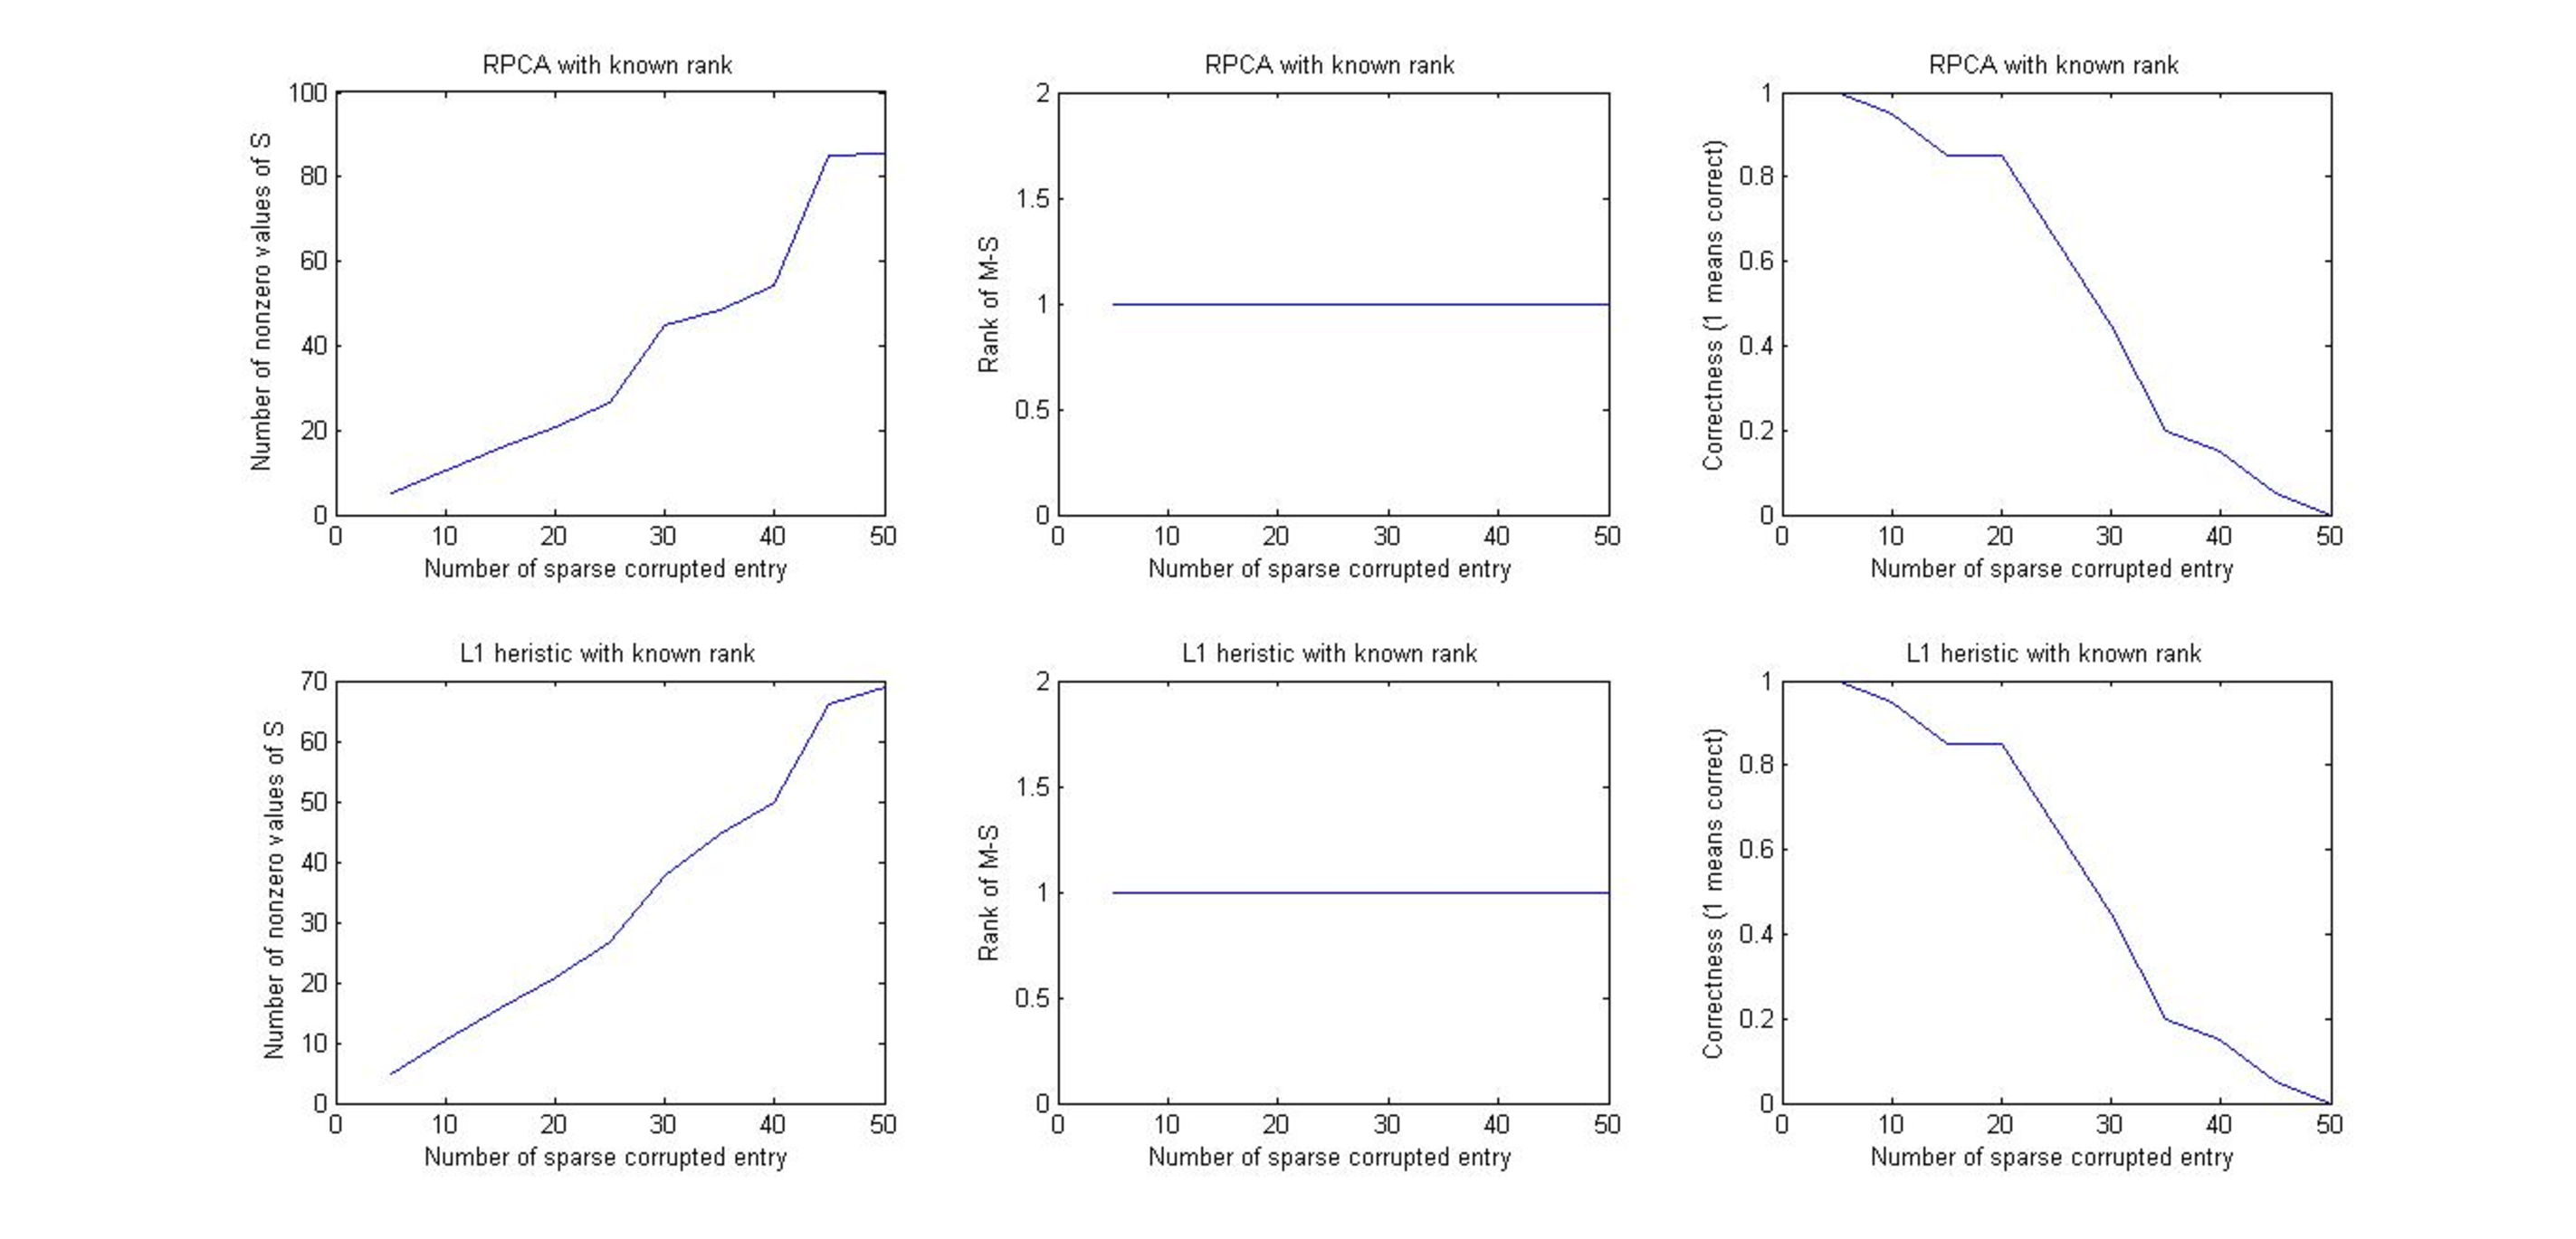
\includegraphics[width=\textwidth]{../figures/compare.pdf}
\label{fig:l1pca_vs_rankone_rpca}
\caption{Comparison of rank one Robust PCA and the $\ell_1$ PCA heuristic in solving rank-one matrix recovery. Both algorithms have similar performance, but $\ell_1$ PCA shows slightly better recovery rate, and its estimated corruption matrix has size of support closer to reality for large supports.}
\end{figure}

If we do not use the rank information in the Robust PCA formulation, the exact recovery performance degrades compared to $\ell_1$ PCA. This is shown in Figure~\ref{fig:l1pca_vs_pure_rpca}

\begin{figure}[h!]
\label{fig:l1pca_vs_pure_rpca}
\centering
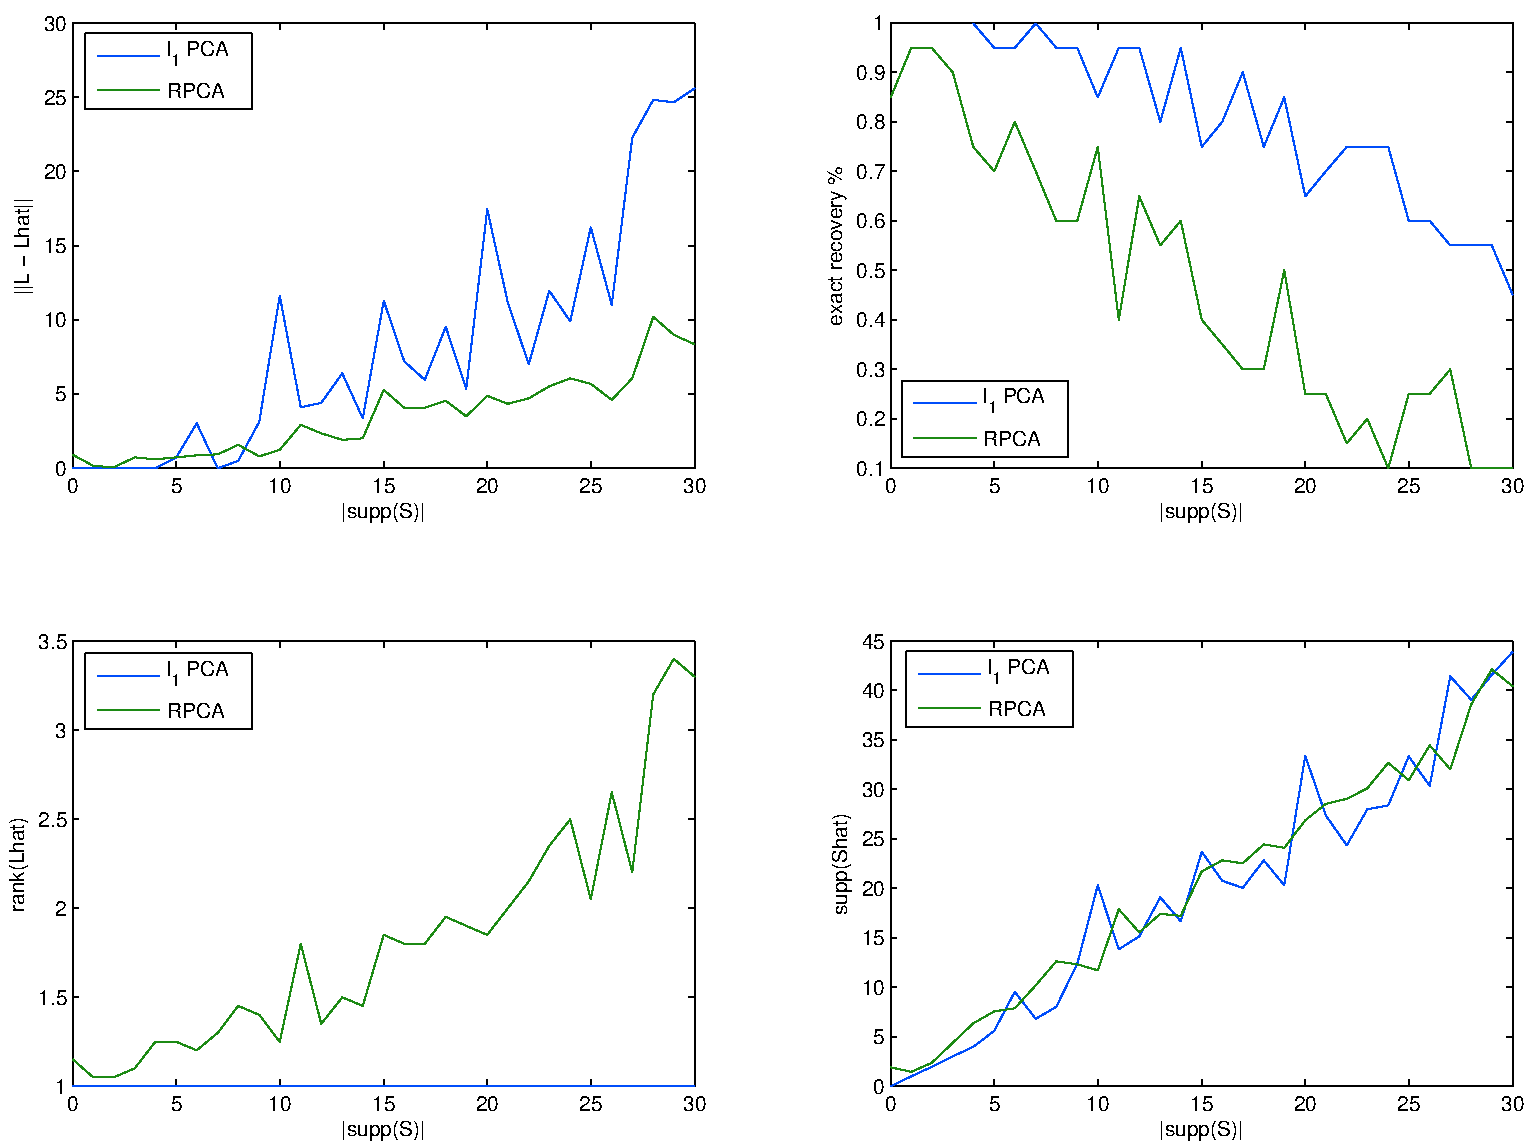
\includegraphics[width=\textwidth]{../figures/l1pca_rk1_rpca_vs_l1pca.pdf}
\caption{Comparison of pure Robust PCA (no rank information) and $\ell_1$ PCA for solving rank one recovery, for increasing sizes of the corruption matrix. $\ell_1$ PCA shows higher exact recovery rates, and lower average error. Observe that the rank of the estimated matrix is increasing in the case of RPCA, but is constant (by construction) in the case of $\ell_1$ PCA.}
\end{figure}


\newpage
%-----------------------------------------------------------------------------------------------------------------------------------------------------------------
\subsection{$\ell_{1}$ PCA heuristics for higher ranks}
One can generalize the $\ell_1$ PCA block coordinate descent algorithms to cases where~$L$ is of known rank~$r \geq 1$, in two different ways depending on what we want to achieve, and on the performance requirements.

\subsubsection{Analysis $\ell_1$ PCA}
In the analysis view of PCA, one seeks to \emph{sequentially} find directions that best explain the data. In the $\ell_2$ case, at each step, we look for a direction $p$ that maximizes the variance along $p$, i.e. $\max_{\|p\|_2 =1} p^TMM^Tp = \max_{\|p\|_2 =1} \|M^Tp\|_2^2$. Equivalently, we look for $p$ that minimizes the distances of the data points $M_i$ to $\mathbf{span}(p)$ ($M_i$ is the $i$-th column of $M$). Indeed, assuming $\|p\|_2 =1$, the projection of data point $M_i$ on $p$ is given by $(M_i^Tp) p$, and the distance of $M_i$ to $\mathbf{span}(p)$ is simply $\|M_i - (M_i^Tp) p\|_2^2 = \|M_i\|_2^2 - (M_i^Tp)^2$. Thus minimizing the sum of the squared distances is equivalent to
\[
\min_{\|p\|_2 = 1} - \sum_i (M_i^Tp)^2 = \max_{\|p\|_2 = 1} \|M^Tp\|_2^2
\]

For a general norm $\|.\|$, minimizing the distance to $\mathbf{span}(p)$ can be written
\[
\min_{q, \|p\|_* = 1} \|M^T - p q^T\|
\]
where $p$ is normalized in the dual sense, and $q_i p$ is the projection of $M_i$ on $p$.

The analysis view of $\ell_1$ PCA leads to a sequential formulation where at each step, a one-dimensional projection of the data is computed
\[
\min_{q_k, \|p_k\|_\infty = 1} \|M^{(k)} - p_kq_k^T\|_1
\]
then the data matrix is updated (the covariance matrix is deflated)
\[
M^{(k+1)} = M^{(k)} - p_kq_k^T
\]
One way to solve this problem is to use block coordinate descent \emph{separately for each pair} $(p_k, q_k)$ (i.e. one block coordinate descent for each step $k$).

\subsubsection{Synthesis $\ell_1$ PCA}
In the synthesis view of PCA, one seeks to find, \emph{simultaneously}, a small set of directions (of size~$r$), or dictionary elements, such that each data point $M_i$ admits a decomposition on that set with low error. This leads to the batch problem
\[
\min_{\|p_k\|_\infty = 1, q_k} \| M - \sum_{k=1}^{r} p_k q_k^T \|_1
\]

that can be solved using block coordinate descent for all vectors $p_k, q_k$
Note that in the case of $\ell_2$ PCA, both views are equivalent and lead to the same solution ($p_k$ is the left singular vector corresponding to the $k$-th largest singular value $\sigma_k$, and $q_k / sigma_k$ is the corresponding right singular vector). However in the general case, these formulations are not equivalent. The synthesis view has slower convergence, since the optimization is done simultaneously on all vectors. The analysis view has faster convergence, but performs poorly compared to the analysis view if the criterion is the reconstruction error $\| M - \sum_{k=1}^{r} p_k q_k^T \|_1$. This is illustrated in the following section.

\newpage
\subsubsection{Numerical results}
We first test the performance of the synthesis $\ell_1$ PCA, for recovering rank-2 $10\times 10$ matrices. The results show that we do have a good performance when the noise is sparse enough.
%
\begin{figure}[h!]
\centering
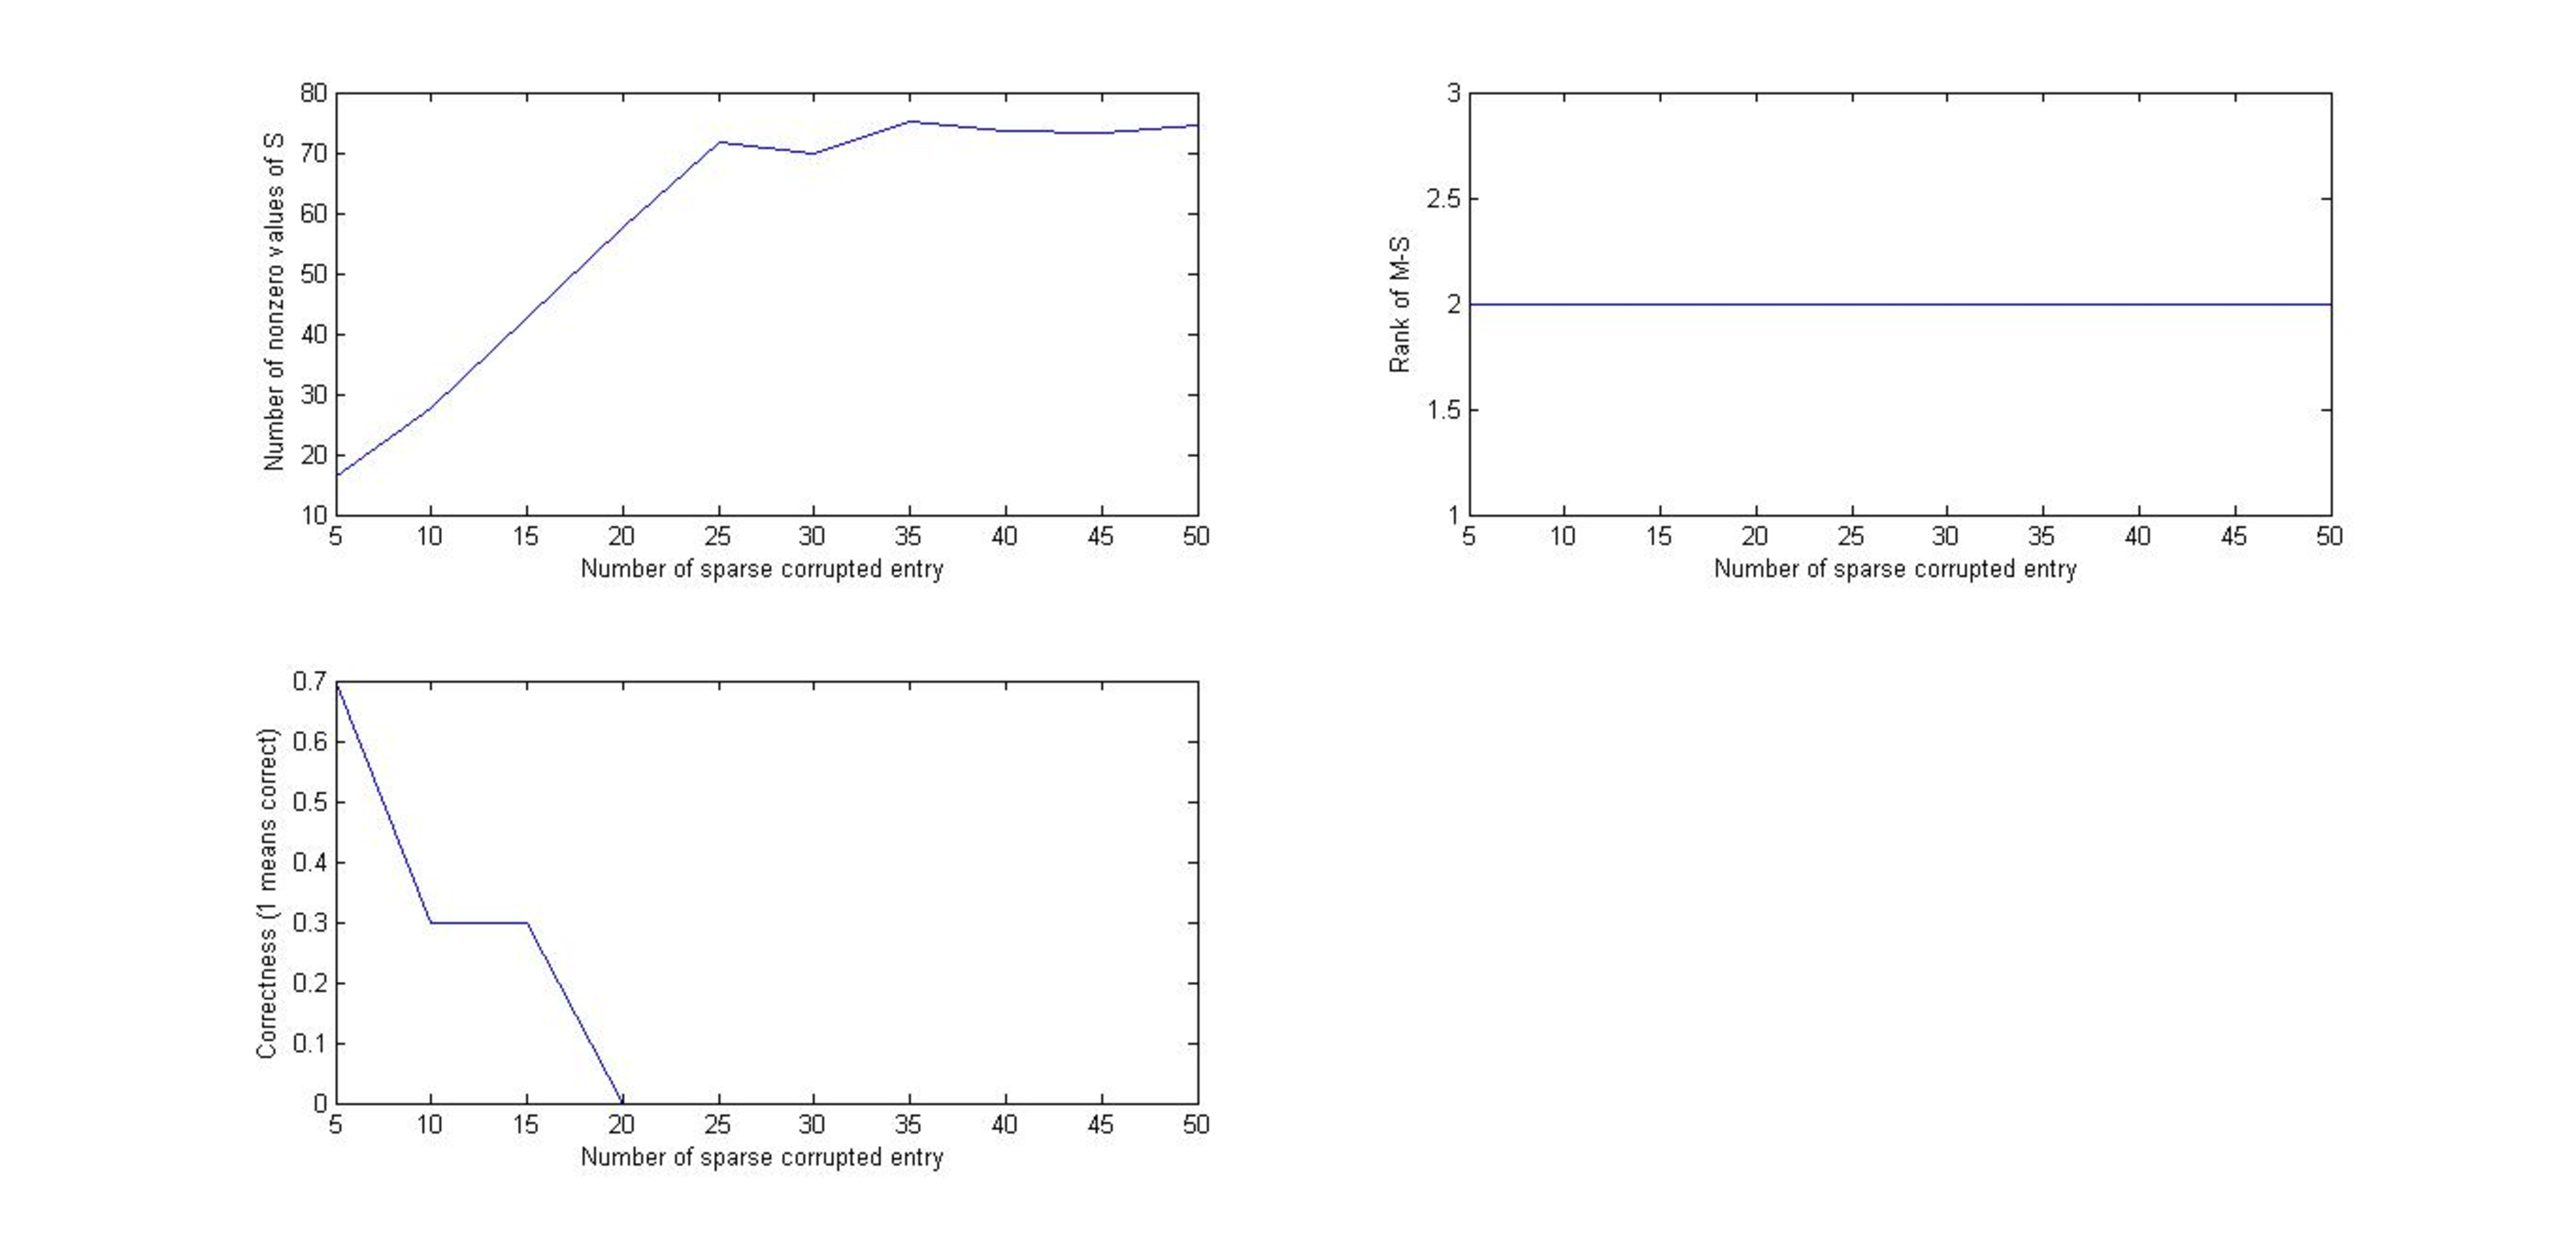
\includegraphics[width=\textwidth]{../figures/rank2case.pdf}
\caption{Performance of synthesis $\ell_1$ PCA in recovering a rank 2 matrix using (batch) block coordinate descent.}
\label{fig:rank2}
\end{figure}

We next compare the performance of the synthesis $\ell_1$ PCA (green), analysis $\ell_1$ PCA (blue), and Robust PCA with no rank information (red). We generate random rank-$r$ $10\times 10$ matrices, and add random uniformly distributed noise. In a first simulation (Figure~\ref{fig:l1pca_by_support}), we fix the rank to be $r = 2$, and vary the size of the support of the corruption matrix $S$. In a second simulation (Figure~\ref{fig:l1pca_by_rank}), we fix the size of the support to be $20$, and vary the rank of $L$. The results show that
\begin{itemize}
\item Synthesis $\ell_1$ PCA performs better than analysis $\ell_1$ PCA, as expected: it achieves higher exact recovery rate, although has comparable average error. However, convergence is much slower. Synthesis $\ell_1$ PCA becomes impractical for large matrices (size of the order of thousand by thousand), but analysis $\ell_1$ PCA still converges fast and yields relatively good recovery rates.
\item The exact recovery rates of RPCA and  $\ell_1$ PCA are comparable, although RPCA achieves lower average error (and slightly better exact recovery, for example, when the rank is $3$). The $\ell_1$ PCA heuristics have an advantage in terms of rank and support of the estimated components: for higher ranks, the $\mathbf{rank}(\hat{L})$ is closer to the original $\mathbf{rank}(L)$, and the size of the support $|\mathbf{supp}(\hat{S})|$ is closer to the original $|\mathbf{supp}(S)|$ (see bottom sub-figures in Figure~\ref{fig:l1pca_by_rank}, original noise support size is $|\mathbf{supp}(S)| = 8$.)
\item The $\ell_1$ PCA heuristics therefore offer some advantages: they allow us to incorporate rank information (we do not see an easy way to add rank information to the RPCA formulation when the rank is strictly greater than one), and offer more robustness when the rank is high.
\end{itemize}
%
\begin{figure}[h!]
\centering
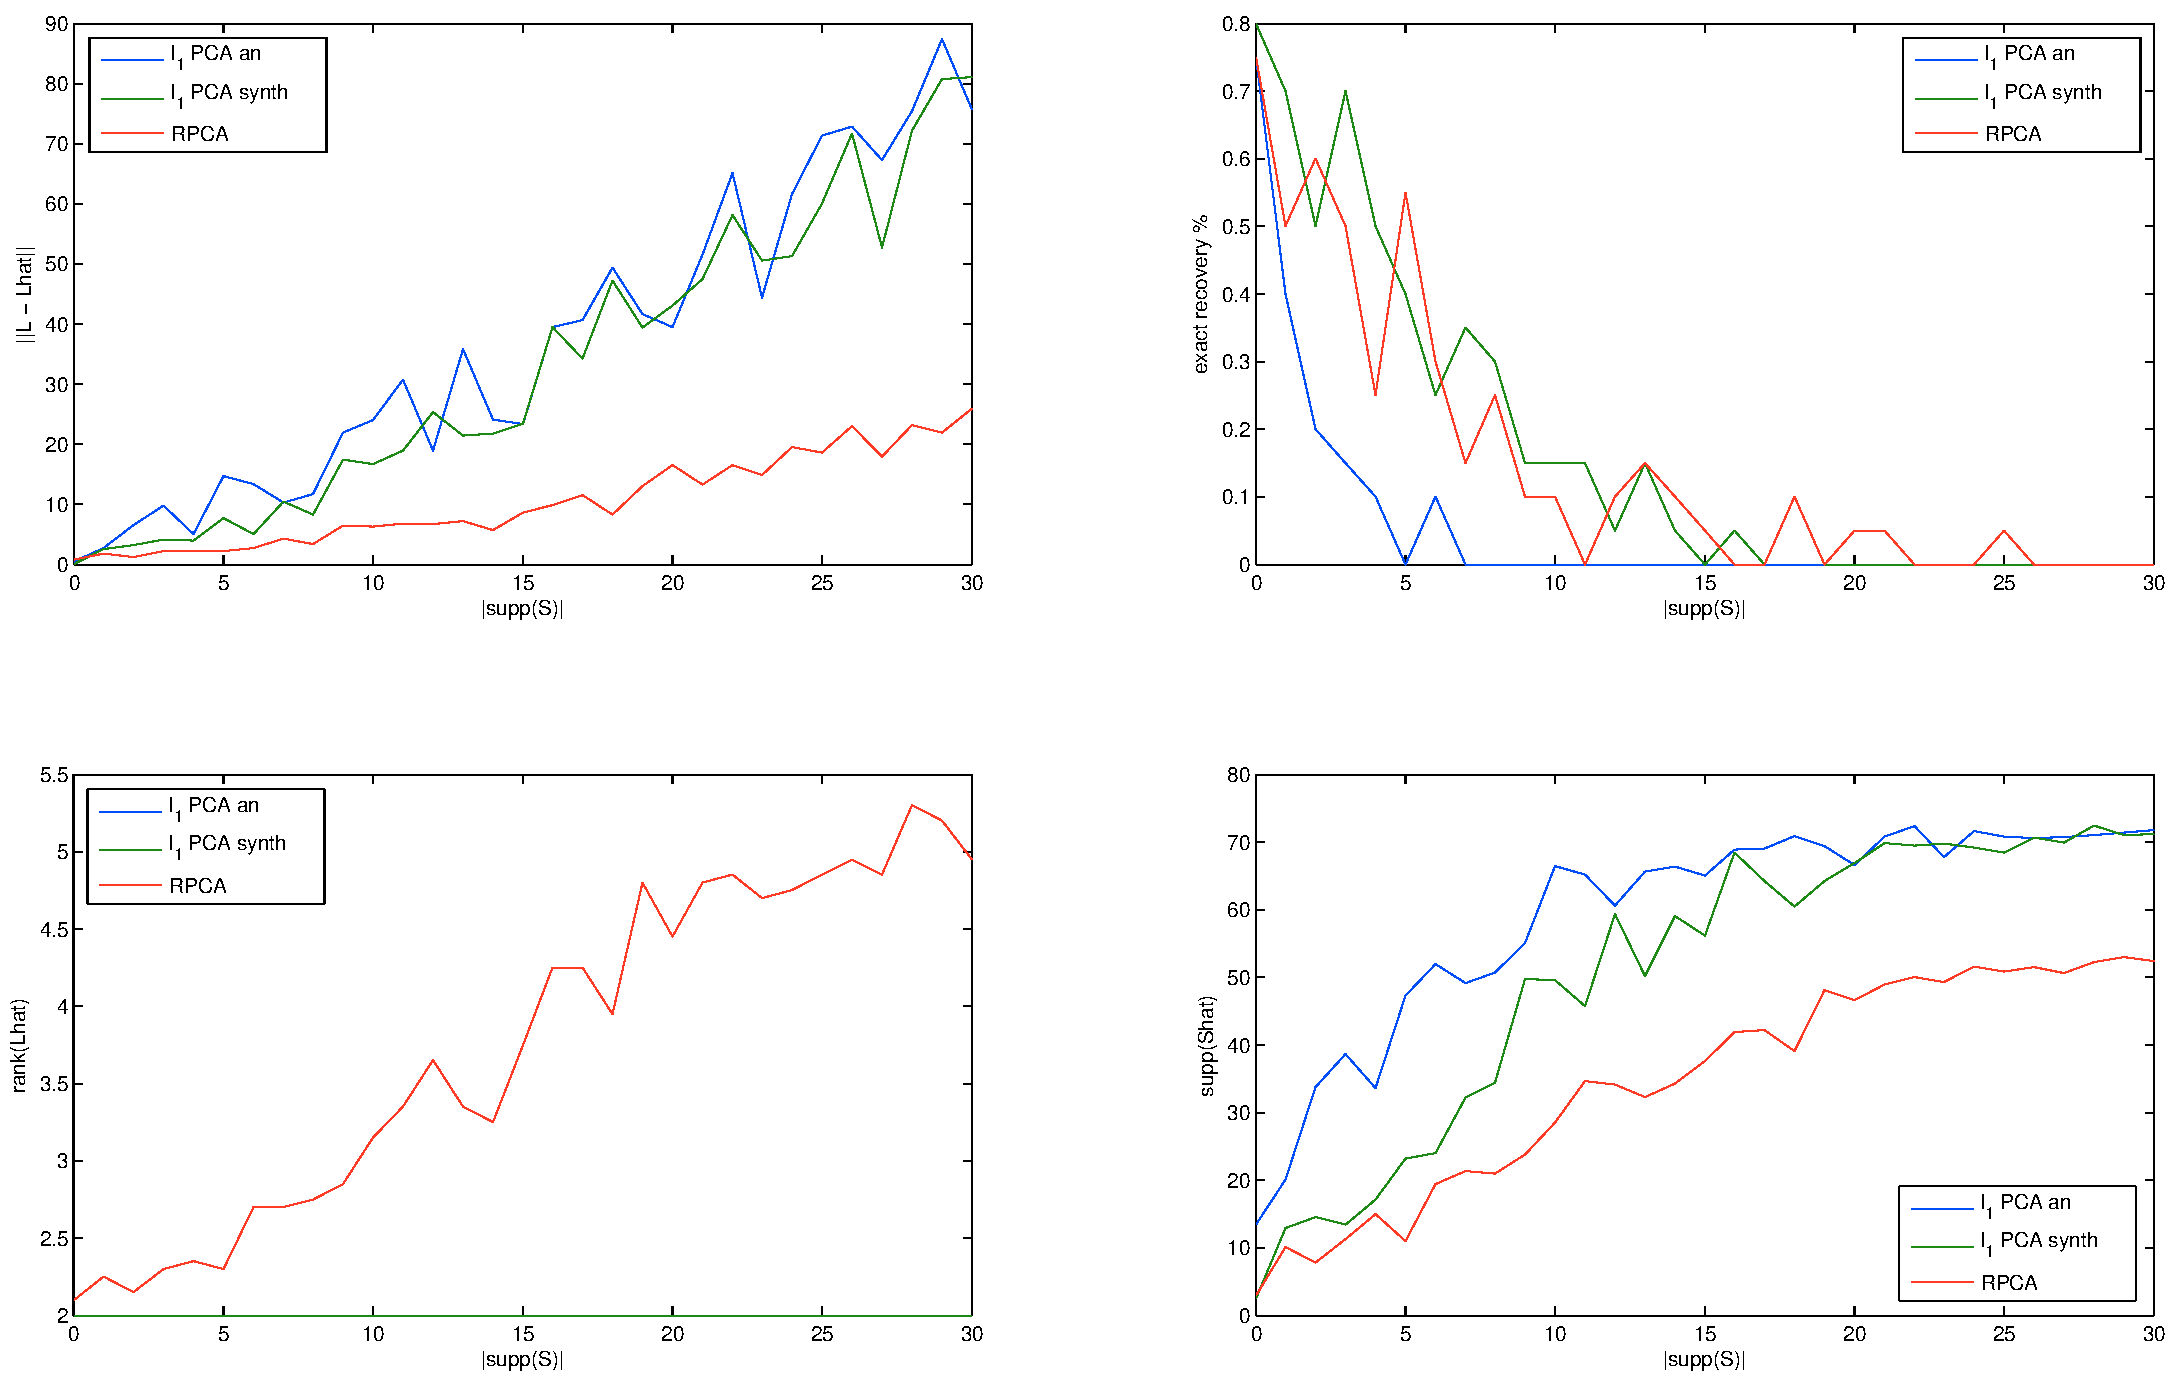
\includegraphics[width=\textwidth]{../figures/l1pca_10x10_rank2_by_support.pdf}
\caption{Analysis $\ell_1$ PCA (blue), synthesis $\ell_1$ PCA (green), and Robust PCA (red) for rank-$2$ recovery, by increasing noise support.}
\label{fig:l1pca_by_support}
\end{figure}

\begin{figure}[h!]
\centering
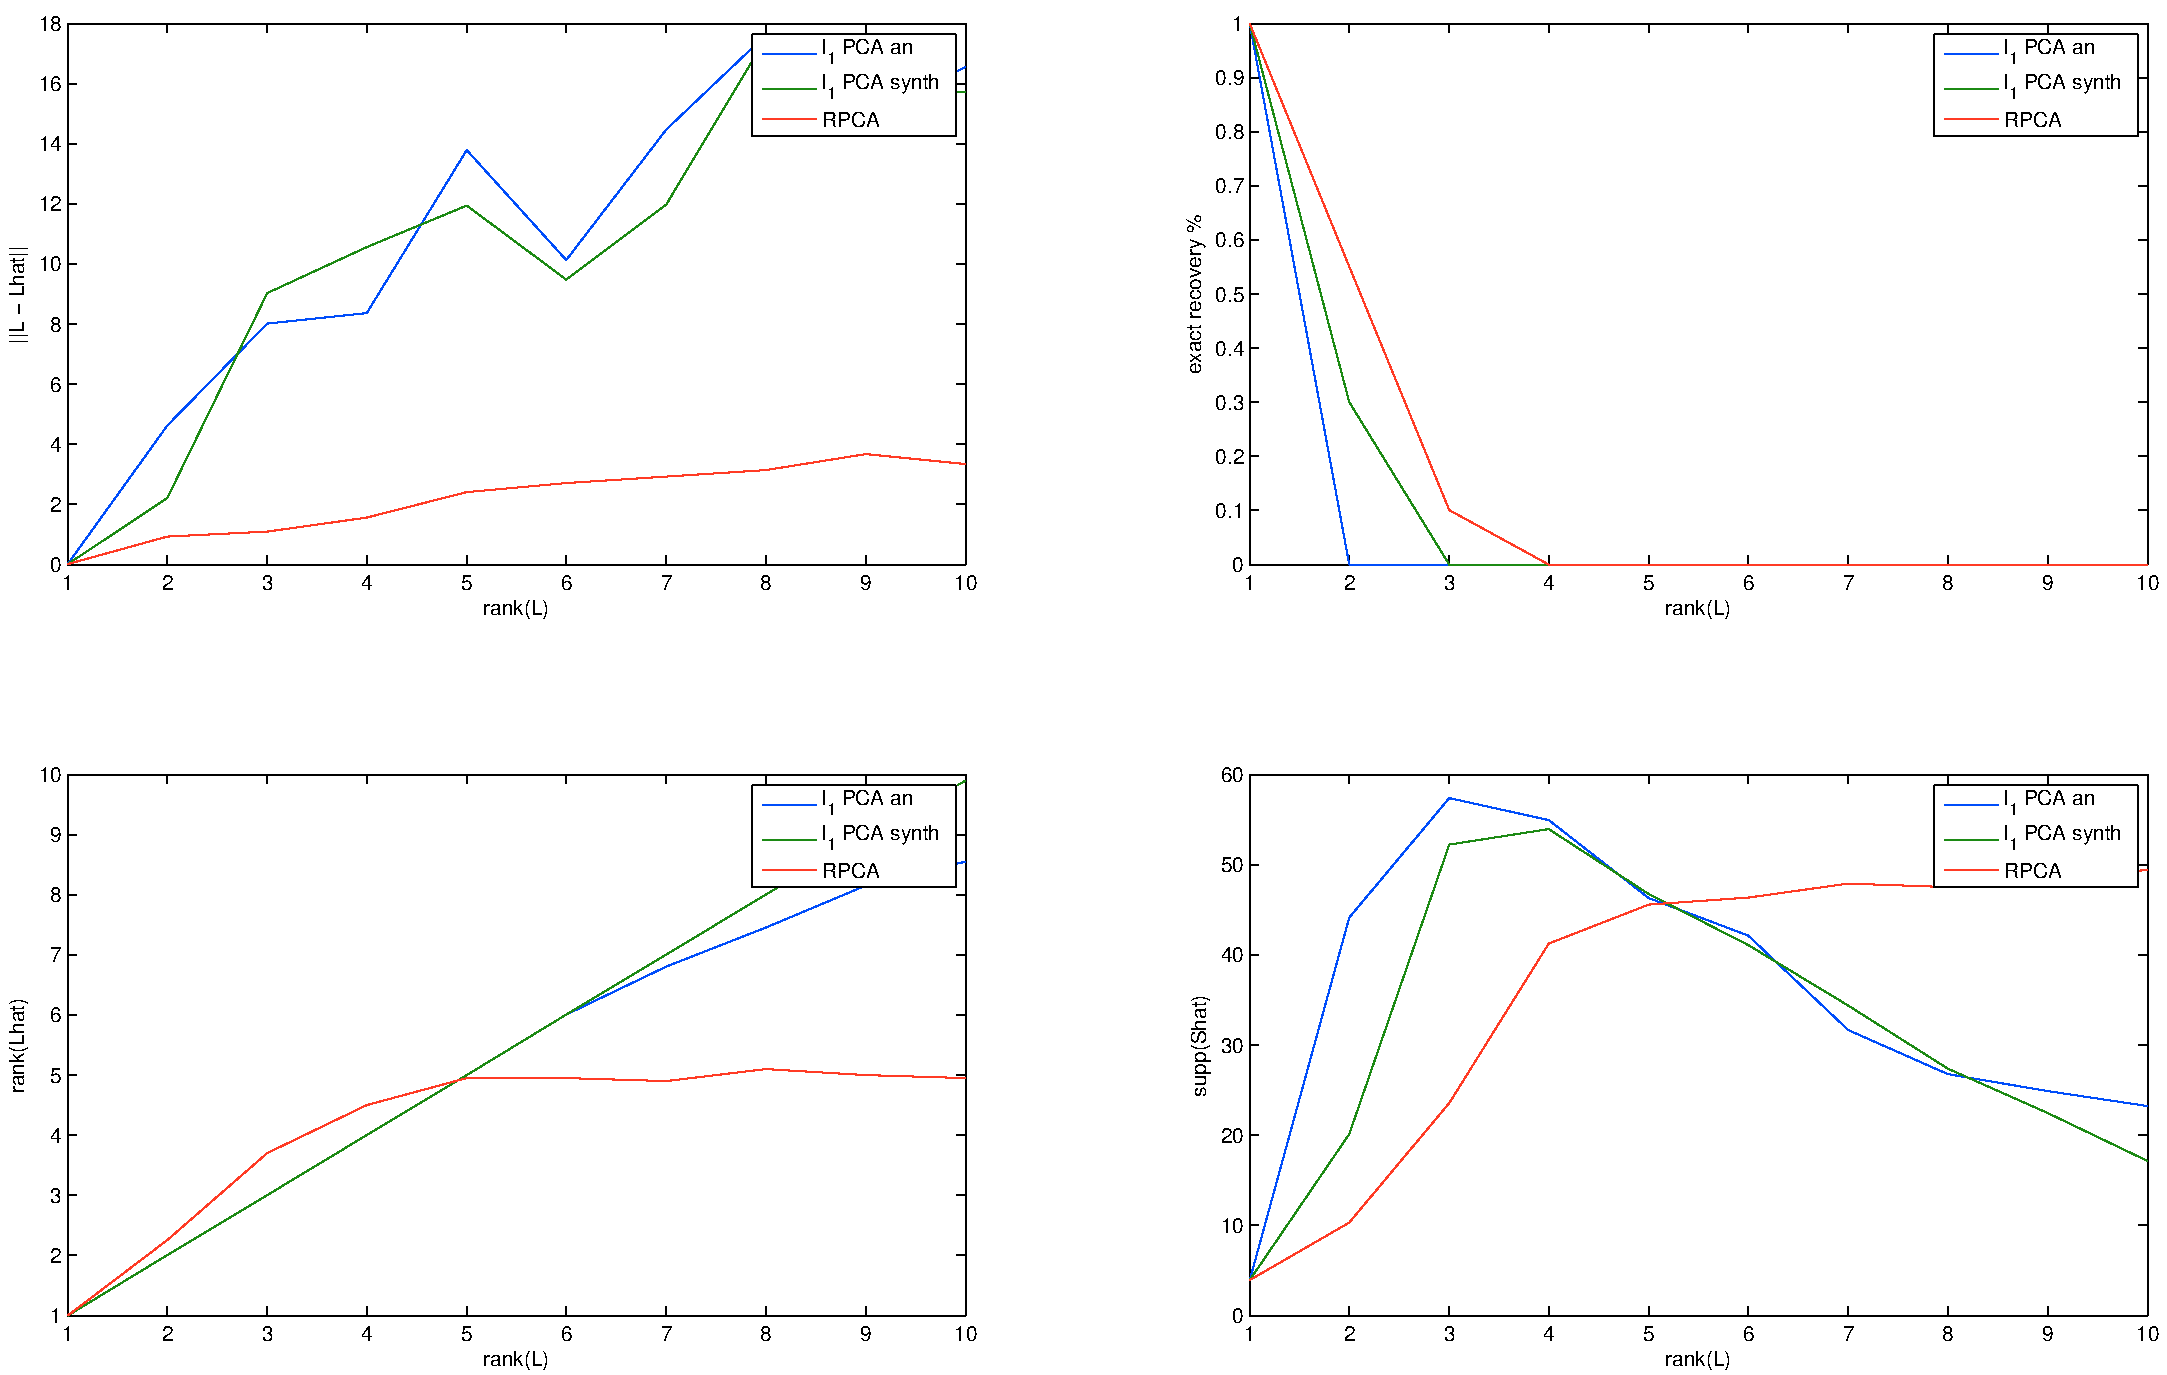
\includegraphics[width=\textwidth]{../figures/l1pca_10x10_support8_by_rank.pdf}
\caption{Analysis $\ell_1$ PCA (blue), synthesis $\ell_1$ PCA (green), and Robust PCA (red) for fixed noise support ($20$), by increasing rank.}
\label{fig:l1pca_by_rank}
\end{figure}

